\documentclass[12pt, a4paper]{article}

\usepackage{array}
\usepackage[portuguese]{babel}
\usepackage{chngpage}
\usepackage{float}
\usepackage[a4paper, margin=2cm]{geometry}
\usepackage{graphicx}
\usepackage{hyperref}
\usepackage{listings}
\usepackage{setspace}
\usepackage{xcolor}

\lstdefinestyle{codestyle}{
    language=c++,
    commentstyle=\color{teal},
    keywordstyle=\color{blue},
    numberstyle=\ttfamily\color{gray},
    stringstyle=\color{red},
    basicstyle=\ttfamily\footnotesize,
    breakatwhitespace=false,
    breaklines=false,
    keepspaces=true,
    numbers=none,
    showspaces=false,
    showstringspaces=false,
    showtabs=false,
    tabsize=4
}
\lstset{style=codestyle}

\title{\Huge \textbf{Computação Gráfica \\ \Large Trabalho Prático -- Fase I}}
\date{2 de março 2025}
\author{Grupo \textbf{\color{red} TODO}}

\begin{document}

\begin{center}
    
\includegraphics[width=0.25\textwidth]{res/cover/EE-C.eps}
\end{center}

\chardef\_=`_
\onehalfspacing
\setlength{\parskip}{\baselineskip}
\setlength{\parindent}{0pt}
\def\arraystretch{1.5}

{\let\newpage\relax\maketitle}
\maketitle
\thispagestyle{empty}

\vspace*{\fill}

\begin{adjustwidth}{-2cm}{-2cm} % These values only need to be large enough to center the table
    \begin{center}
        \begin{tabular}{>{\centering}p{0.25\textwidth}
                        >{\centering}p{0.25\textwidth}
                        >{\centering}p{0.25\textwidth}
                        >{\centering\arraybackslash}p{0.25\textwidth}}
            
\includegraphics[width=3.5cm]{res/cover/A104437.png} &
            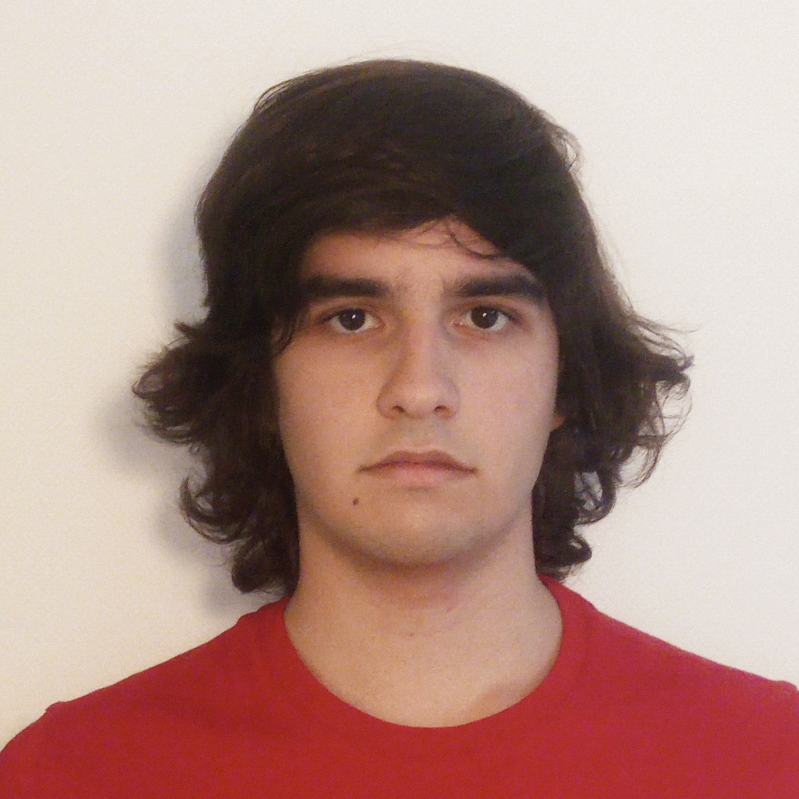
\includegraphics[width=3.5cm]{res/cover/A104348.png} &
            
\includegraphics[width=3.5cm]{res/cover/A90817.png} &
            
\includegraphics[width=3.5cm]{res/cover/A104179.png} \\

            Ana Oliveira & Humberto Gomes & Mariana Cristino & Sara Lopes \\
            A104437      & A104348        & A90817           & A104179
        \end{tabular}
    \end{center}
\end{adjustwidth}

\pagebreak

\begin{abstract}
    \textbf{\color{red} TODO - resumo}
\end{abstract}

\section{\emph{Generator}}

\textbf{\color{red} TODO - \emph{generator}}

\section{\emph{Engine}}

\subsection{Criação da janela}

Para a criação da janela, a biblioteca GLFW foi utilizada \cite{glfw}, escolhida principalmente pela
sua API moderna. Ao contrário do GLUT \cite{glut}, utilizado nas aulas práticas da UC, a API do GLFW
não obriga a guardar o estado da aplicação em variáveis globais para que os métodos associados à
janela lhe possam aceder. Isto possibilita a criação de abstrações RAII em torno da janela criada, o
que por sua vez permite a utilização das várias funcionalidades de C++ para gestão automática de
memória. Ademais, a API do GFLW também permite um maior controlo sobre o ciclo de resposta a eventos
e renderização.

Já na primeira fase do projeto, optou-se por utilizar uma versão do OpenGL mais atual do que a que é
utilizada nas aulas práticas, o \emph{core profile} do OpenGL 4.6. Apesar do seu uso exigir um maior
esforço na primeira fase, com a utilização obrigatória de VBOs e de \emph{shaders}, esta versão
suporta mais funcionalidades do que as versões anteriores, permite obter um melhor desempenho, e é
suportada por depuradores como RenderDoc \cite{renderdoc}. Para utilizar esta versão de OpenGL, um
\emph{loader} é necessário, e o GLAD \cite{glad} foi escolhido devido ao seu elevado grau de
personalização.

\subsection{Comportamento da \emph{engine}}

O primeiro passo na execução da \emph{engine} é a criação da janela e do seu contexto OpenGL. Este é
necessário para os passos seguintes: a leitura da cena, onde é necessário criar VBOs para os
modelos 3D, a instanciação dos eixos do sistema de coordenadas, também suportados por VBOs, e a
criação dos \emph{shaders} de vértices e de fragmentos. Uma vez que os VBOs e os \emph{shaders} não
são um objetivo da primeira fase deste trabalho, o seu funcionamento só será descrito em detalhe num
relatório futuro.

Estando inicializada a \emph{engine}, segue-se um ciclo em que a janela reage a eventos e desenha os
seus conteúdos. Neste ciclo, são suportados os eventos de passagem de tempo, necessidade de
atualizar os conteúdos da janela, e redimensionamento da janela. Para se subscrever a um evento,
basta sobrescrever o seu método correspondente na classe \texttt{Window}:

\begin{lstlisting}

virtual void onUpdate(float time, float timeElapsed) = 0;
virtual void onRender() = 0;
virtual void onResize(int width, int height) = 0;
\end{lstlisting}

De momento, apenas os métodos \texttt{onRender} e \texttt{onResize} são utilizados. Nestes,
desenham-se os conteúdos da janela e atualiza-se a matriz de projeção da câmara, respetivamente. Em
relação ao processo de renderização, este consiste no envio da matriz da câmara para o \emph{shader}
de vértices, na renderização dos eixos usando \texttt{glDrawArrays}, e na iteração por todos os
objetos da cena, usando \texttt{glDrawElements} para desenhar cada um. No futuro, serão adicionados
métodos de resposta a eventos de \emph{input} do utilizador, que o permitirão executar ações como,
por exemplo, mover a câmara.

\section{Resultados obtidos}

\textbf{\color{red} TODO - resultados}

\section{Conclusão e Trabalho Futuro}

\textbf{\color{red} TODO - conclusão}

\begingroup
\section{Bibliografia}
\renewcommand{\section}[2]{}

\begin{thebibliography}{9}
    \bibitem{glfw}
        "An OpenGL library."{} GLFW. Accessed: Feb. 27, 2025. [Online.] Available:
        \url{https://www.glfw.org}
    \bibitem{glut}
        "About."{} The freeglut project. Accessed: Feb. 27, 2025. [Online.] Available:
        \url{https://freeglut.sourceforge.net/}
    \bibitem{renderdoc}
        "RenderDoc."{} RenderDoc Accessed: Feb. 28, 2025. [Online.] Available:
        \url{https://renderdoc.org/}
    \bibitem{glad}
        "Glad - Multi-Language GL/GLES/EGL/GLX/WGL Loader-Generator based on the official specs."{}
        Feb. 28, 2025. [Online.] Available: \url{https://glad.dav1d.de/}
\end{thebibliography}
\endgroup

\end{document}
